%% Included in decks: slidemage-manual, slidemage-manual-copy
%%

% SlideMage manual, chapter "Working in SlideMage": the slide editor, on the
% standardframe demo slide (tools/manual/make_screenshots.py). Writing and
% seeing the result here; slide 1b2 explains the slide-level buttons and the
% AI buttons.
\setSlideVersion{1-1-0}
\begin{standardframe}{The slide editor}
	\small
	A slide's source opens in the slide editor, from the deck editor or from the \emph{Slide name search} in the main window. You write the LaTeX directly: the	source uses syntax highlighting, aided by toolbar buttons. To see the result you do not have to compile the whole deck.
	\par\smallskip
	\begin{columns}[T,onlytextwidth]
		\begin{column}{0.44\linewidth}
			{\setlength{\fboxsep}{0pt}\fcolorbox{c_primary_gray}{white}{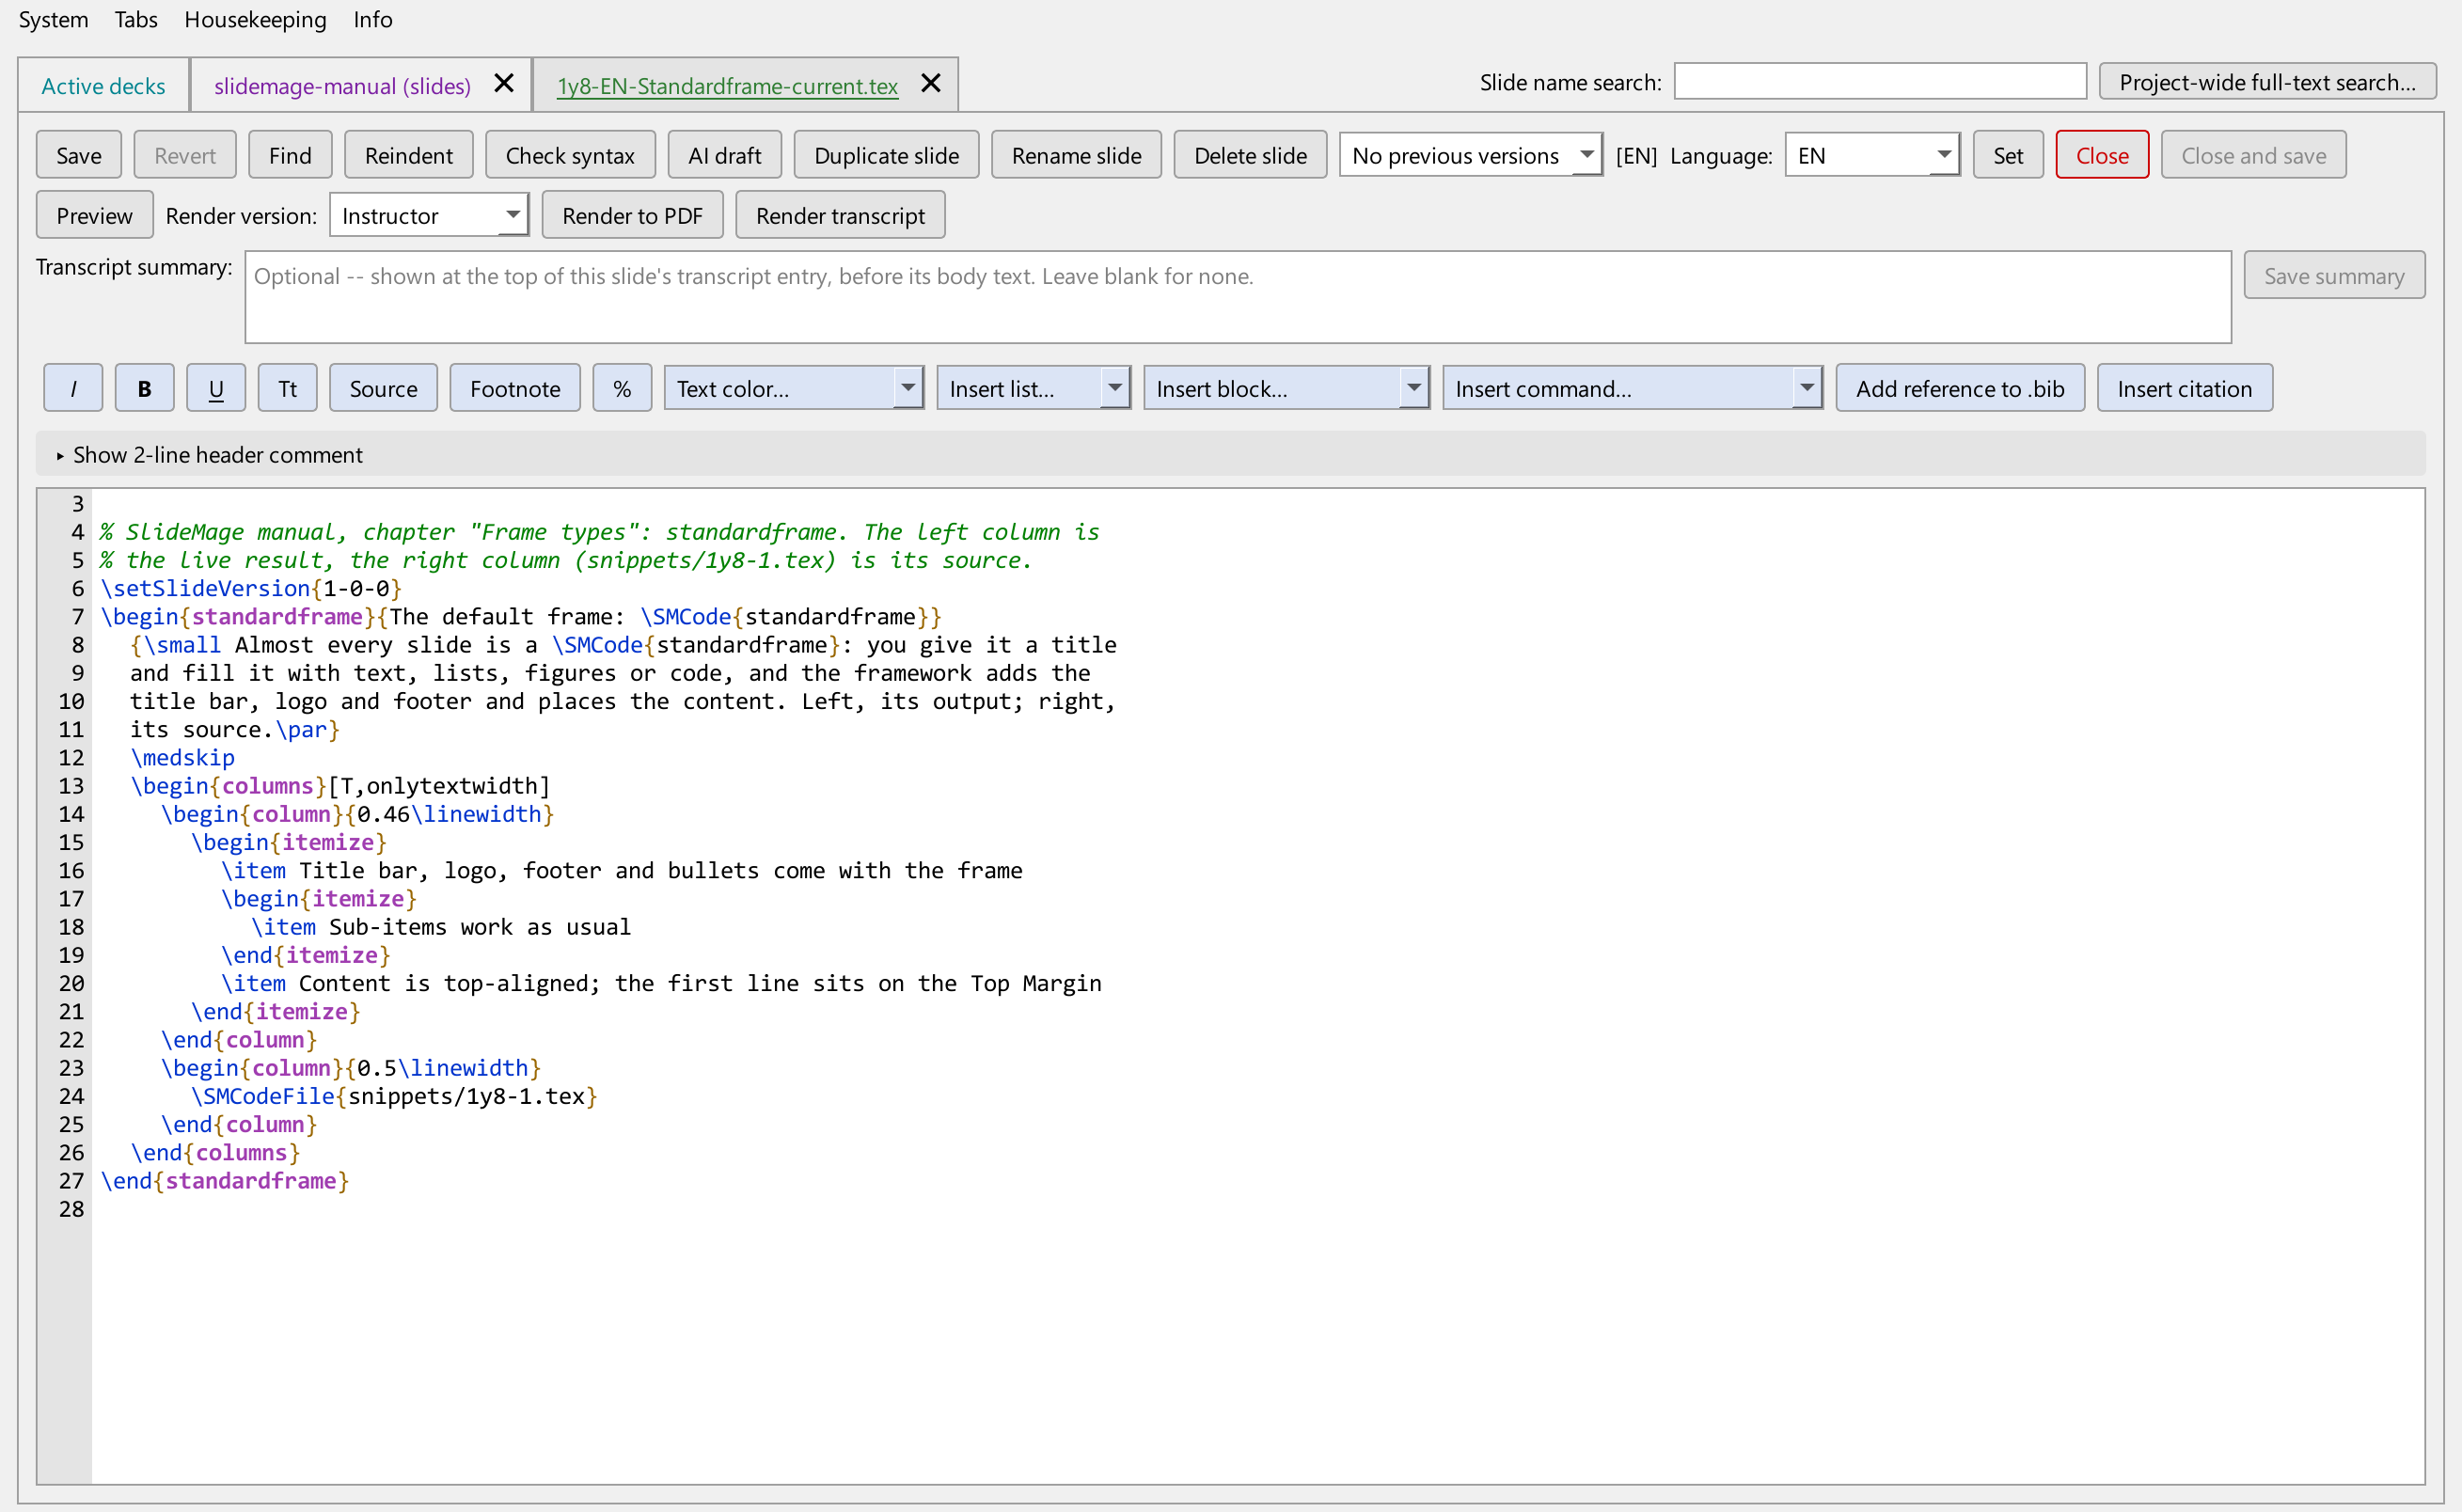
\includegraphics[width=\dimexpr\linewidth-0.8pt\relax]{media/screenshot-slidemage-slide-editor.png}}}
		\end{column}
		\begin{column}{0.54\linewidth}
			\shrinklists{2}
			\begin{itemize}
				\item \textbf{Writing.} The tinted buttons above the source insert styles, footnotes, colors, lists, blocks, commands and citations; \emph{Find}, \emph{Reindent} and \emph{Revert} search and replace, tidy indentation, and drop changes since the last save.
				\item \textbf{Seeing the result.} \emph{Render to PDF} compiles the text in the editor, saved or not. \emph{Preview} shows the picture from the last compile of the saved slide (instant, maybe outdated). \emph{Render transcript} shows its transcript entry.
				\item \textbf{Transcript summary.} An optional sentence at the head of the slide's transcript entry.
			\end{itemize}
		\end{column}
	\end{columns}
\end{standardframe}
